%set the master document for easy compilation
%!TEX root = ../D3_5_3.tex

\section{F2.13: manageTIU\_output}\label{s:F2.13}

\todo[inline]{section and corresponding subsections have to be completed}

\subsection{Component Requirements}

\begin{longtable}{p{.25\textwidth}p{.7\textwidth}}
\toprule
Component name			& manageTIU\_output \\
\midrule
Link to SCADE model		& {\footnotesize \url{http://???}} \\
\midrule
SCADE designer			& Bernd Hekele, DB Netz AG \\
\midrule
Description				& [Brief description of the components functionality] \\
\midrule
Input documents	& 
Subset-026, Chapter ?.?\newline
Subset-026, Chapter ?.?\newline
Subset-026, Chapter ?.?.?\\
\midrule
Safety integrity level		& 4 \\
\midrule
Time constraints		& [If applicable description of time constraints, otherwise n/a] \\
\midrule
API requirements 		& [If applicable description of API requirements, otherwise n/a] \\
\bottomrule
\end{longtable}


\subsection{Interface}

An overview of the interface of component manageTIU\_output is shown in Figure~\ref{f:manageTIUOutput}. The inputs and outputs are described in detail in Section~\ref{s:manageTIUOutput_inputs} respectively \ref{s:manageTIUOutput_outputs}. Subcomponents are described in Section~\ref{s:manageTIUOutput_subcomponents}.

\begin{figure}
\center
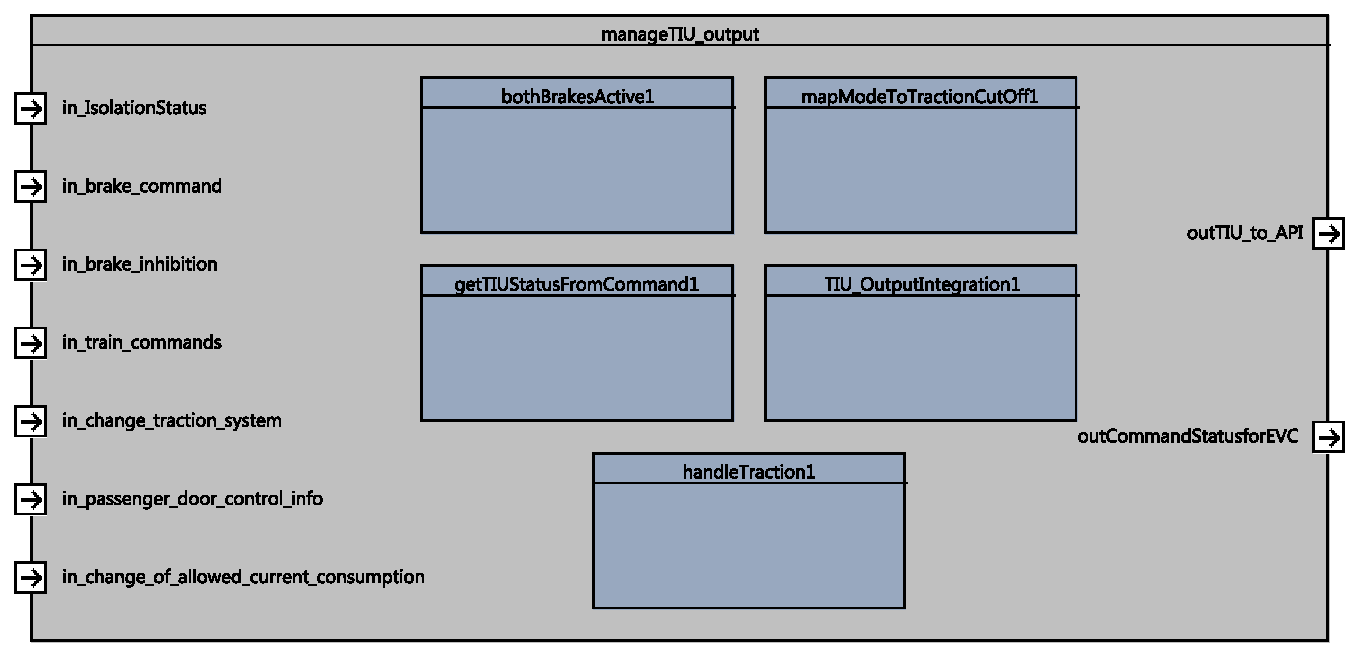
\includegraphics[width=\textwidth]{images/F2_13_manageTIU_output.pdf}
\caption{manageTIU\_output SysML diagram.}\label{f:manageTIUOutput}
\end{figure}


\subsubsection{Inputs}\label{s:manageTIUOutput_inputs}

\paragraph{[Input 1 name]}

\begin{longtable}{p{.25\textwidth}p{.7\textwidth}}
\toprule
Input name				& [Name of the input] \\
\midrule
Description				& [Brief description of the input] \\
\midrule
Source					& [Name of the source component] \\ 
\midrule
Type					& [Type of the input] \\
\midrule
Valid range of values	& [Complete list of valid values] \\
\midrule
Behaviour when value is at boundary	& [Description of components behaviour when input value is at boundary] \\
\midrule
Behaviour for values out of valid range	& [Description of components behaviour when input value is out of valid range] \\
\midrule
Behaviour when value is erroneous, absent or unwanted (i.e. spurious) & [Description of components behaviour when value is erroneous, absent or unwanted (i.e. spurious)] \\
\bottomrule
\end{longtable}


\paragraph{[Input 2 name]}

\begin{longtable}{p{.25\textwidth}p{.7\textwidth}}
\toprule
Input name				& [Name of the input] \\
\midrule
Description				& [Brief description of the input] \\
\midrule
Source					& [Name of the source component] \\ 
\midrule
Type					& [Type of the input] \\
\midrule
Valid range of values	& [Complete list of valid values] \\
\midrule
Behaviour when value is at boundary	& [Description of components behaviour when input value is at boundary] \\
\midrule
Behaviour for values out of valid range	& [Description of components behaviour when input value is out of valid range] \\
\midrule
Behaviour when value is erroneous, absent or unwanted (i.e. spurious) & [Description of components behaviour when value is erroneous, absent or unwanted (i.e. spurious)] \\
\bottomrule
\end{longtable}


\subsubsection{Outputs}\label{s:manageTIUOutput_outputs}

\paragraph{[Output 1 name]}

\begin{longtable}{p{.25\textwidth}p{.7\textwidth}}
\toprule
Output name				& [Name of the output] \\
\midrule
Description				& [Brief description of the output] \\
\midrule
Destination				& [Name of the destination component(s)] \\ 
\midrule
Type					& [Type of the output] \\
\midrule
Valid range of values	& [Complete list of valid values] \\
\midrule
Behaviour when value is at boundary	& [Description of components behaviour when output value is at boundary] \\
\midrule
Behaviour for values out of valid range	& [Description of components behaviour when output value is out of valid range] \\
\midrule
Behaviour when value is erroneous, absent or unwanted (i.e. spurious) & [Description of components behaviour when value is erroneous, absent or unwanted (i.e. spurious)] \\
\bottomrule
\end{longtable}


\paragraph{[Output 2 name]}

\begin{longtable}{p{.25\textwidth}p{.7\textwidth}}
\toprule
Output name				& [Name of the output] \\
\midrule
Description				& [Brief description of the output] \\
\midrule
Destination				& [Name of the destination component(s)] \\ 
\midrule
Type					& [Type of the output] \\
\midrule
Valid range of values	& [Complete list of valid values] \\
\midrule
Behaviour when value is at boundary	& [Description of components behaviour when output value is at boundary] \\
\midrule
Behaviour for values out of valid range	& [Description of components behaviour when output value is out of valid range] \\
\midrule
Behaviour when value is erroneous, absent or unwanted (i.e. spurious) & [Description of components behaviour when value is erroneous, absent or unwanted (i.e. spurious)] \\
\bottomrule
\end{longtable}

\subsection{Subcomponents}\label{s:manageTIUOutput_subcomponents}

\subsubsection{handleTraction}
%set the master document for easy compilation
%!TEX root = ../D3_5_3.tex

\paragraph{Component Requirements}

\begin{longtable}{p{.25\textwidth}p{.7\textwidth}}
\toprule
Component name			& handleTraction \\
\midrule
Link to SCADE model		& {\footnotesize \url{http://???}} \\
\midrule
SCADE designer			& Bernd Hekele, DB Netz AG \\
\midrule
Description				& [Brief description of functionality] \\
\midrule
Input documents	& 
Subset-026, Chapter ?.?\newline
Subset-026, Chapter ?.?\newline
Subset-026, Chapter ?.?.?\\
\midrule
Safety integrity level	& 4 \\
\midrule
Time constraints		& [If applicable description of time constraints, otherwise n/a] \\
\midrule
API requirements 		& [If applicable description of API requirements, otherwise n/a] \\
\bottomrule
\end{longtable}


\paragraph{Interface}

For an overview of the interface of this internal component we refer to the SCADE model (cf.~link above) respectively the SCADE generated documentation.

\subsubsection{manageTIU\_output}
%set the master document for easy compilation
%!TEX root = ../D3_5_3.tex

\paragraph{Component Requirements}

\begin{longtable}{p{.25\textwidth}p{.7\textwidth}}
\toprule
Component name			& manageTIU\_output \\
\midrule
Link to SCADE model		& {\footnotesize \url{http://???}} \\
\midrule
SCADE designer			& Bernd Hekele, DB Netz AG \\
\midrule
Description				& [Brief description of functionality] \\
\midrule
Input documents	& 
Subset-026, Chapter ?.?\newline
Subset-026, Chapter ?.?\newline
Subset-026, Chapter ?.?.?\\
\midrule
Safety integrity level	& 4 \\
\midrule
Time constraints		& [If applicable description of time constraints, otherwise n/a] \\
\midrule
API requirements 		& [If applicable description of API requirements, otherwise n/a] \\
\bottomrule
\end{longtable}


\paragraph{Interface}

For an overview of the interface of this internal component we refer to the SCADE model (cf.~link above) respectively the SCADE generated documentation.